\section{The ATARI ST line of personal computers}
\label{sec:atarist}

The US-American hardware and software company \gls{ATARI} started out by creating very successful video game consoles for pubs and other public spaces. At that time, hardware and software of these machines were still tightly integrated. The first game of this kind was \textbf{Pong}, a simple two-player game derived from tennis.

After that, ATARI created multiple consumer video-game consoles, which brought computer games directly into individual households. In 1979, they announced their first general purpose 8-bit computers, the \textit{400} and the \textit{800}.

In 1985, ATARI introduced their next generation of home computers: The \textbf{ATARI ST}\footnote{\url{https://archive.org/details/atarist}}. They were relatively inexpensive and achieved wide adoption on the Western European market.

The first computers of the series (260ST, 520ST, 520ST+) featured a dedicated sound chip, a \acrshort{rom} cartridge slot, \acrshort{midi} input and output ports, an external \acrshort{crt} monitor, a parallel port for a printer, a serial port for a modem, an external floppy disk drive, a connector for an external hard drive, and ports for a mouse and a joystick. The keyboard was integrated into the case of the machine. The later computers of the series (1040ST) had a floppy disk drive built in \cite{vogt2021History}.

The \acrfull{midi} ports turned the ATARI ST into a machine that was useful in music studios and other kinds of real-time digital signal processing such as experiments in physics or electrical engineering in academic settings\footnote{\url{https://archive.org/details/MIDIMusi1986}}.

The name \textbf{ST} refers to the sixteen/thirty-two \gls{bit} \acrfull{isa} of the \acrfullpl{cpu}, which were from the \acrfull{m68k}. These chips used the 16-bit \gls{word} as their fundamental unit of data storage but used 32-bit addresses for the main memory.

Similar to the \textit{Apple Lisa} computer, the ATARI ST was part of the first generation of computers to be distributed with a graphical user interface as part of the operating system. This development is ultimately derived from the 1968 ``mother of all demos'' by Douglas Engelbart. With his \textbf{oN-Line System}, Engelbart and colleagues had demonstrated the first prototype of the \textbf{WIMP} paradigm; making use of Windows, Images, Menus, and a (Mouse)Pointer \cite{english1967display}.

\begin{figure}[h]
    \centering
    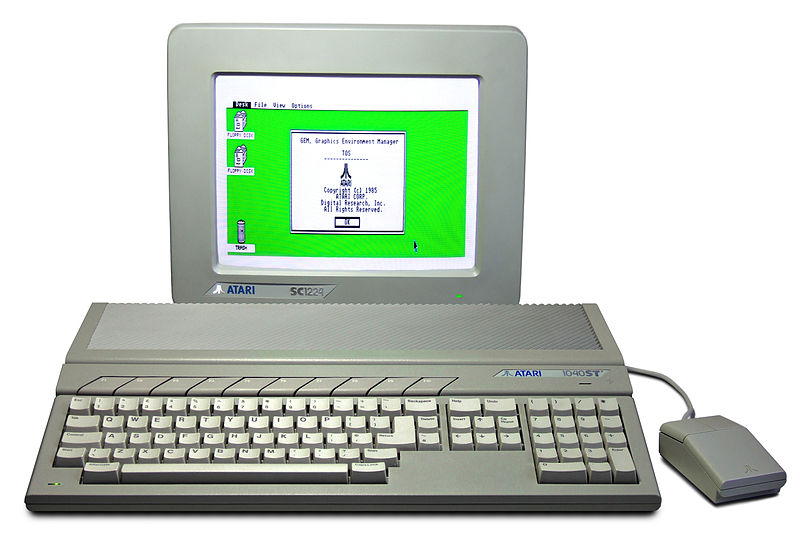
\includegraphics[width=\columnwidth]{img/800px-Atari_1040STf.jpg}
    \caption{Picture of an Atari 1040ST\textsuperscript{F}; \copyright Bill Bertram, 2006, \url{https://commons.wikimedia.org/wiki/File:Atari_1040STf.jpg}}
    \label{fig:atari_1040st}
\end{figure}

\subsection{Recovering floppy disks today}
\label{sec:floppy-disks}

%\funfact{My research into this topic started with a box of floppy disks marked Signum! in my parents' basement}
The very first versions of the ST line had neither a hard disk for persistent storage nor a built-in drive for removable media. Consumers had to buy an additional floppy disk drive to load the programs that they wanted to use and to store the data that they generated.

In those days, a consumer would insert the floppy disk for a program like \textit{Signum!}, start the program, which would load the complete program into the main memory, insert another floppy disk with the files they wanted to edit, and use the open program to work with those files.

The type of floppy disk used with the ATARI ST computers were 3.5'' (inches), with a storage capacity of about 720 kilobytes. Later advances in disk technology allowed for so-called \textit{double-density} disks with about 1.4 megabytes in storage space.

To analyze or recover documents created with the \Signum{} word processor, it's very likely that we need to read such disks because that is where files were saved at the time. As modern computers do not have a floppy disk drive anymore, the first step is to acquire an external drive that can be connected via USB cable. This enables me to make a complete copy of the disk that we can work on without putting any more strain on the original physical disk.

I used the \texttt{ddrescue} command line tool available for the Linux operating system to perform that recovery. The result is single image file per disc; the conventional file extensions for these images is \textit{*.st} \cite{archiveteam:stdisc}.

\begin{lstlisting}[style=BashInputStyle]
$ ddrescue -n /dev/sdb myfloppy.st myfloppy.log
\end{lstlisting}

As with modern disks or flash drives, an ST-compatible floppy disk consists of a hierarchy of files and folders. To that end, the disk image is structured according to a file-system, in this case \textbf{FAT12}. Fortunately, the FAT12 file system is not exclusive to the ST and a modern Linux system still supports it with only minor differences relating to the last-edited timestamps on the files.

Hence, I can \textit{mount} a floppy disk image into our main file-system using a simple \texttt{mount} command, provided the directory \texttt{/mnt/floppy} exists:

\begin{lstlisting}[style=BashInputStyle]
$ mount -ro myfloppy.st /mnt/floppy
\end{lstlisting}

I can now use the files from the floppy disk for any subsequent processing that may be necessary, without the risk of damaging the original disks.

\subsection{Using a machine emulator}
\label{sec:emulator}

One useful tool in analyzing the Signum! word processor is the ability to run the original software in a machine emulator. Emulation, in this case, refers to the simulation of the original \acrshort{m68k} \acrshort{cpu} and associated peripherals of an ST computer using software that runs on a modern computer.

Thanks to a large number of people interested in retro-computing, there are multiple emulators available for the ATARI ST as well as associated archives of software to run on these computers. 

The most important component of this setup is the \textbf{\acrshort{tos}-\acrshort{rom}}, that is the \acrlong{rom} representation of \acrlong{tos}. This piece of software was distributed as a built-in storage chip in the original ST computers so it's not really hardware that can be simulated. This is also the most problematic component of the system, because neither Atari, Inc. nor its legal successors have released the copyright to it.

However, there are a number of alternatives:
\acrlong{ash} published the \textbf{MagiC} operating system in 1992. It is a direct replacement for the original \acrshort{tos} and adds new features such as multitasking. It was later incorporated into the \textit{MagiCMac} and \textit{MagiCPC} emulators, that embeds the \acrshort{os} into a program running on Macs and PCs.
The \textbf{EmuTOS} project has also developed an alternative but compatible operating system based on the original GEMDOS sources from Digital Research, that were released under a permissive license around the year 2000 \cite{emuTOSHistory}. This system is available for free under the GPL license.

As I am using a \textit{debian GNU/Linux} system for this research, I chose the \textbf{Hatari} emulator \cite{hatari}, which is readily available as an extension package for my operating system.

Using that system, I could install a copy of \textit{Signum!2}, which is amazingly still available for purchase on the ASH website\footnote{\url{https://www.ashshop.biz/diverses/atari/textverarbeitung/874/signum-2-download}}.

\subsection{TOS - The Operating System}

The operating system of the ATARI ST computers is mostly adapted from products by \gls{DRI}, a company that created the successful \acrshort{cpm} operating system, originally designed for 8-bit microcomputers.

As detailed in \textit{The documentation for TOS}\funfact{The TOS Guide is maintained by the FreeMINT project, aiming to bring a modern operating system to ATARI-ST compatible hardware} \cite{tos.hyp}, the TOS consists of multiple components that work together to create the full operating system:

\begin{description}
    \item[GEM] This is the user-facing name of the full graphical operating system. It is the name of a product by Digital Research and presents a set of windows, icons and menus to the user, who can interact with them using a mouse.
    \item[VDI] The Virtual Device Interface is the low-level graphics system that allows a programmer to display text, images or lines on the screen.
    \item[AES] The Application Environment Services are the high-level parts of the GEM that allow a programmer to define windows and menus.
    \item[GEMDOS] The GEM Disc Operating System is the standard library of functions for a GEM program. It includes subroutines relating to loading and saving files, managing memory or processes or accessing the network.
    \item[BIOS] This Basic Input-Output System is the lower half of a standard operating system. It provides the hardware-specific subroutines that the (GEM)DOS needs to work.
    \item[XBIOS] This eXtended BIOS is a collection of subroutines that provide advanced control of the additional subsystems of the ST, such as the sound chip, the MIDI ports, the keyboard and the printer.
\end{description}

\subsection{The GEM User Interface by Digital Research Inc.}

The original GEM System allows only one application to run at any one time. An application consists of a menu bar, a main background window and a set of floating windows or dialogs.

The default application, which is launched whenever the system is started, is the Desktop or \textbf{Desk}. This application provides access and overview to the installed drives and includes a drag-and-drop file manager. To start a program such a Signum!, you would put in the appropriate floppy disk, double click on the corresponding icon on the desktop, navigate to the folder that contains the \texttt{SIGNUM2.PRG} executable and start the programm by, again, double-clicking the icon.

\begin{figure}[h]
    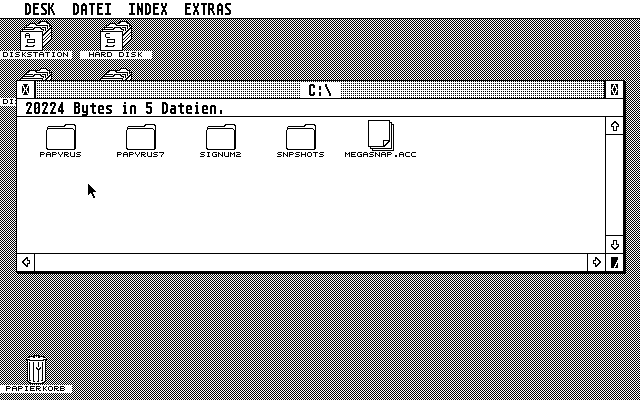
\includegraphics[width=\columnwidth]{img/SNAP2.png}
    \caption{Screenshot of the GEM Desktop Application. \textbf{MEGASNAP.ACC} is an example for an accessory. It can be used to take screenshots like this one.}
\end{figure}

There was one important exception to the rule of allowing only a single application to run at a time: So called \glspl{accessory} are programs that have a file extension of \texttt{ACC}, and which are loaded when the computer is started, provided they are stored at the root of the disk that is inserted while the computer is starting.